\chapter{Methode}
In dit hoofdstuk wordt het ontwerp en de realisatie van de ontworpen pipet besproken. Hierbij worden de verschillende onderdelen behandeld, als ook de gemaakte keuzes.

\section{Conceptueel ontwerp}
\subsection{Literatuurstudie}
De Literatuurstudie bestond voor een groot deel uit het bestuderen van beschikbare patenten. Patenten zoals\ \cite{RN16} en\ \cite{RN17} beschrijven analoge pipetten. Deze worden nog manueel bediend en hebben een relatief eenvoudige werking. Deze patenten waren belangrijk om de basiswerking van moderne pipetten te begrijpen. Ze tonen namelijk aan dat deze pipetten met één eenvoudige zuigerwerking werken. Dit is een belangrijke stap bij het ontwerp van de automatische pipet.
\\\textit{Zie \autoref{sec: Analoge pipetten} voor verdere toelichting betreffende de werking.}
\\[12pt]Verder werden de patenten \ \cite{RN35},\ \cite{RN36} en\ \cite{RN38} bestudeerd. Deze patenten beschrijven de werking van een, motorisch aangedreven, elektronische pipet. In het geval van\ \cite{RN36} en\ \cite{RN38} wordt niet toegelicht welk type motor gebruikt wordt. In het geval van\ \cite{RN35} wordt er vermeld dat er voor een stappermotor is gekozen. Deze patenten tonen aan dat de zuigerwerking van een pipet met een stappermotor kan gebeuren en dat deze met een hoge precisie kunnen werken. Ook dit is een belangrijke stap in het ontwerp van de automatische pipet.

\section{Hardware ontwerp}
Dit onderdeel behandelt de keuzes betreffende de hardware in dit project. De onderdelen die ge-3D-print zijn werden ontworpen in Autodesk Inventor en geprint met Prusa Mk3S en Mk4 printers.

\subsection{Muurelementen}
Zoals eerder vernoemd is voor het hardware ontwerp gekozen voor een modulaire oplossing. Dit laat toe om de verschillende onderdelen onafhankelijk van elkaar te ontwikkelen en indien nodig aan te passen. Dit maakt het in de toekomst ook mogelijk om dit ontwerp uit te breiden tot bijvoorbeeld een meerkanaals systeem. De verschillende modules worden geplaatst over geleidestaven, zoals in\ \autoref{fig:geleidestaven} te zien is. Deze geleidestaven zorgen ervoor dat de verschillende modules correct uitgeleind en geplaatst worden.
\\[12pt]De eerste ontwerpiteraties focusten zich hoofdzakelijk op het ontwerp van de muren. Deze zijn in PLA geprint. Aangezien de muren weinig structurele lasten moeten dragen is PLA een geschikte keuze. In de latere iteraties zijn de muren verdund en zijn de vlakken verdwenen zoals in \autoref{fig:hollowwalls} te zien is. Dit maakt de muren lichter en goedkoper. De muren zijn ook in verschillende hoogtes ontworpen met een geparametriseerd model. 
\\[12pt]Het afgeleverde model bestaat uit twee muurelementen van 40mm en een muurelement van 30mm. De twee elementen van 40mm voorzien ruimte voor de slag van de zuiger. Het muurelement van 30mm voorziet ruimte voor de askoppeling.
\\[12pt]\begin{minipage}[t]{0.49\textwidth}
    \vspace{0pt}
    \begin{figure}[H]
        \centering
        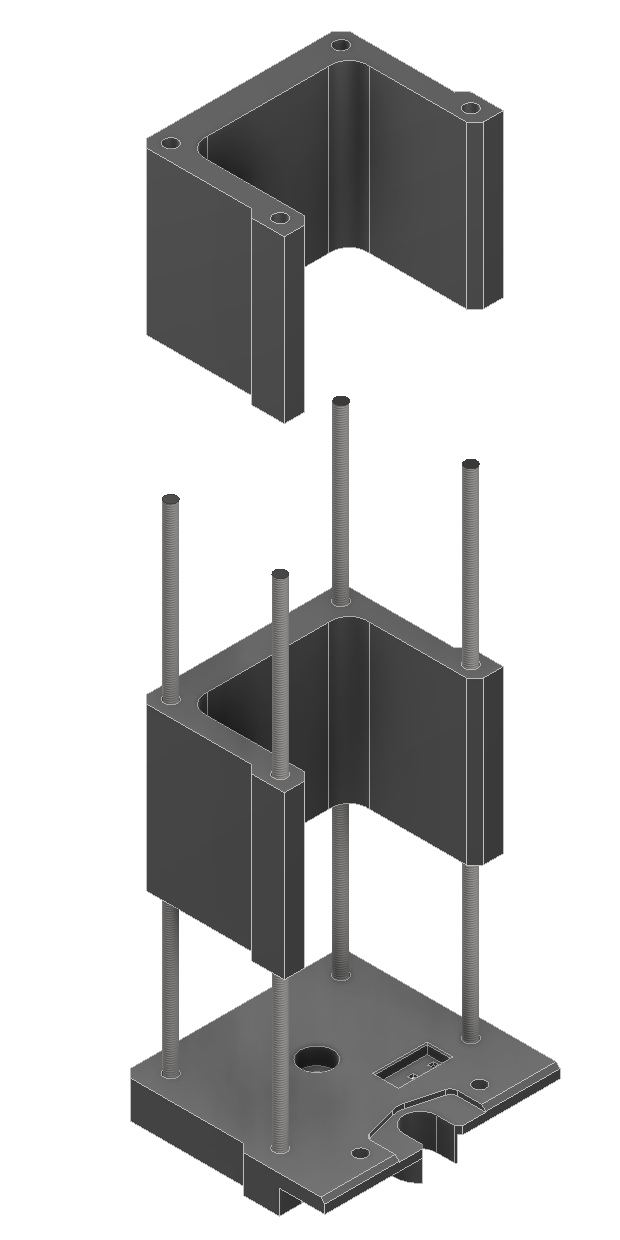
\includegraphics[height=6cm]{figures/GuidesDemonstration.png}
        \caption{Demonstratie van de geleidestaven.}\label{fig:geleidestaven}
    \end{figure}
\end{minipage}
\begin{minipage}[t]{0.49\textwidth}
    \vspace{0pt}
    \begin{figure}[H]
        \centering
        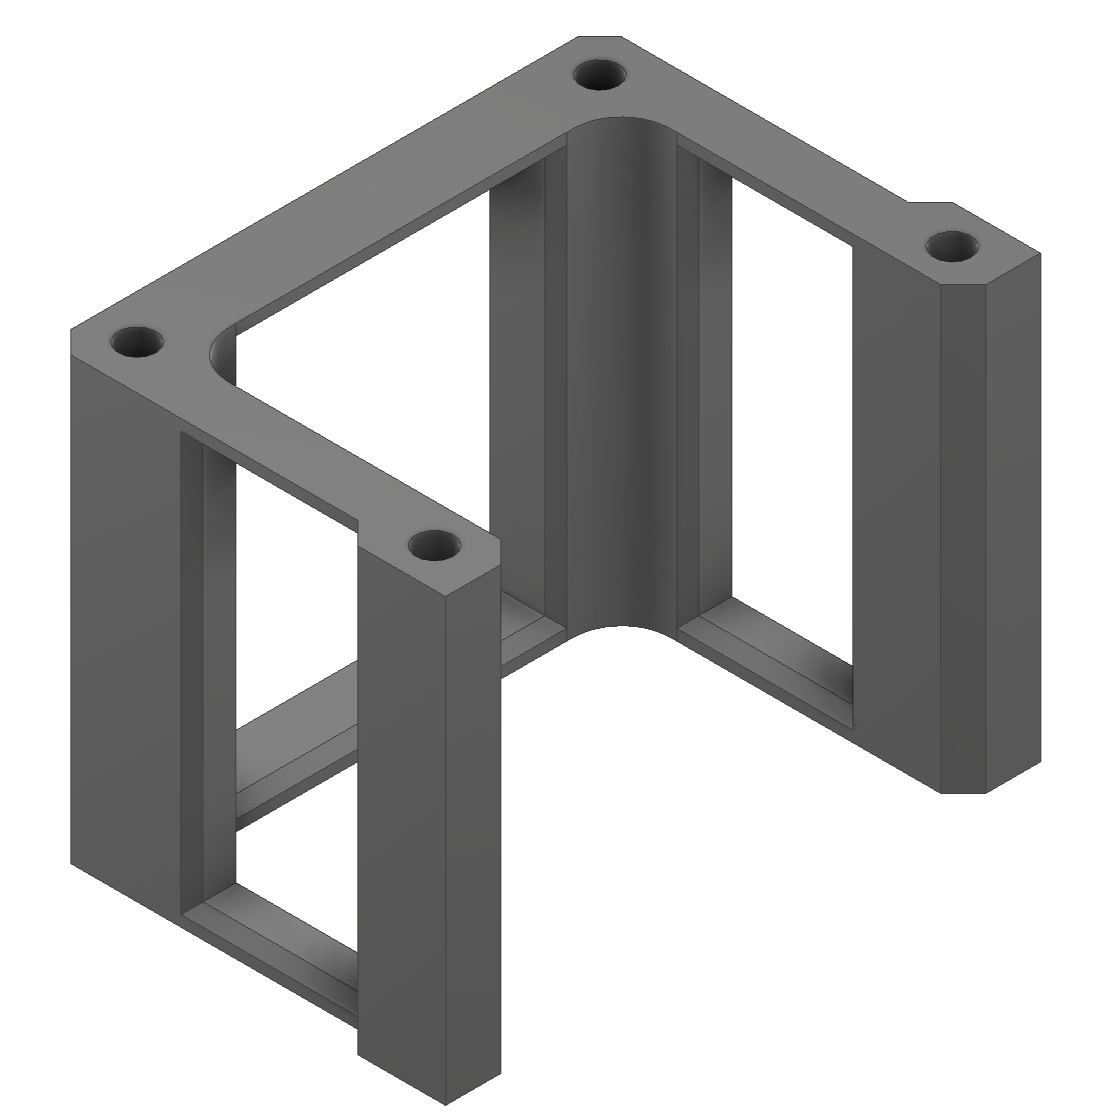
\includegraphics[height=6cm]{figures/Walls_1_w.png}
        \caption{Lichtere muren.}\label{fig:hollowwalls}
    \end{figure}
\end{minipage}\\

\subsection{Bodemplaat en geleidestaven}
De muurelementen en geleidestaven worden op de bodemplaat gemonteerd. De bodemplaat is hiervoor voorzien van gaten waar de geleidestaven doorheen kunnen. Onderaan de geleidestaven bevinden zicht twee tegengedraaide schroeven. Dit wordt bijvoorbeeld toegepast bij de montage van verkeerslichten zoals te zien in \autoref{fig:verkeerslichten}. Dit is een effectieve oplossing die gebruikt kan worden om ge-3D-printte elementen extra te versterken, alsook om de elementen in kleinere onderdelen te bevestigen en daarna aan te spannen. Zo wordt het in\ \cite{RN40} meerdere keren gebruikt.
\\[12pt]De tegengedraaide moeren (type ISO 4032-M3) passen in hiervoor voorziene gaten zoals te zien is in\ \autoref{fig:counterrotated}. Deze gaten bestaan uit twee trappen. De onderste trap heeft een zeshoekigevorm, gebaseerd op de afmetingen van de moer. De moer past net in dit gat maar kan slechts zeer weinig roteren. De tweede moer staat hier dan sterk tegenaan gedraaid zodat deze ook niet zal roteren. De twee trap van het gat is een cilindrisch gat waarin de moer vrij kan roteren. Deze rotatie is echter niet wenselijk, het gat is enkel voorzien zodat de eerste moer, ogeacht de oriëntatie van de tweede moer, in het hexagonale gat kan worden ingebracht.
\\[12pt]\\[12pt]\begin{minipage}[t]{0.49\textwidth}
    \vspace{0pt}
    \begin{figure}[H]
        \centering
        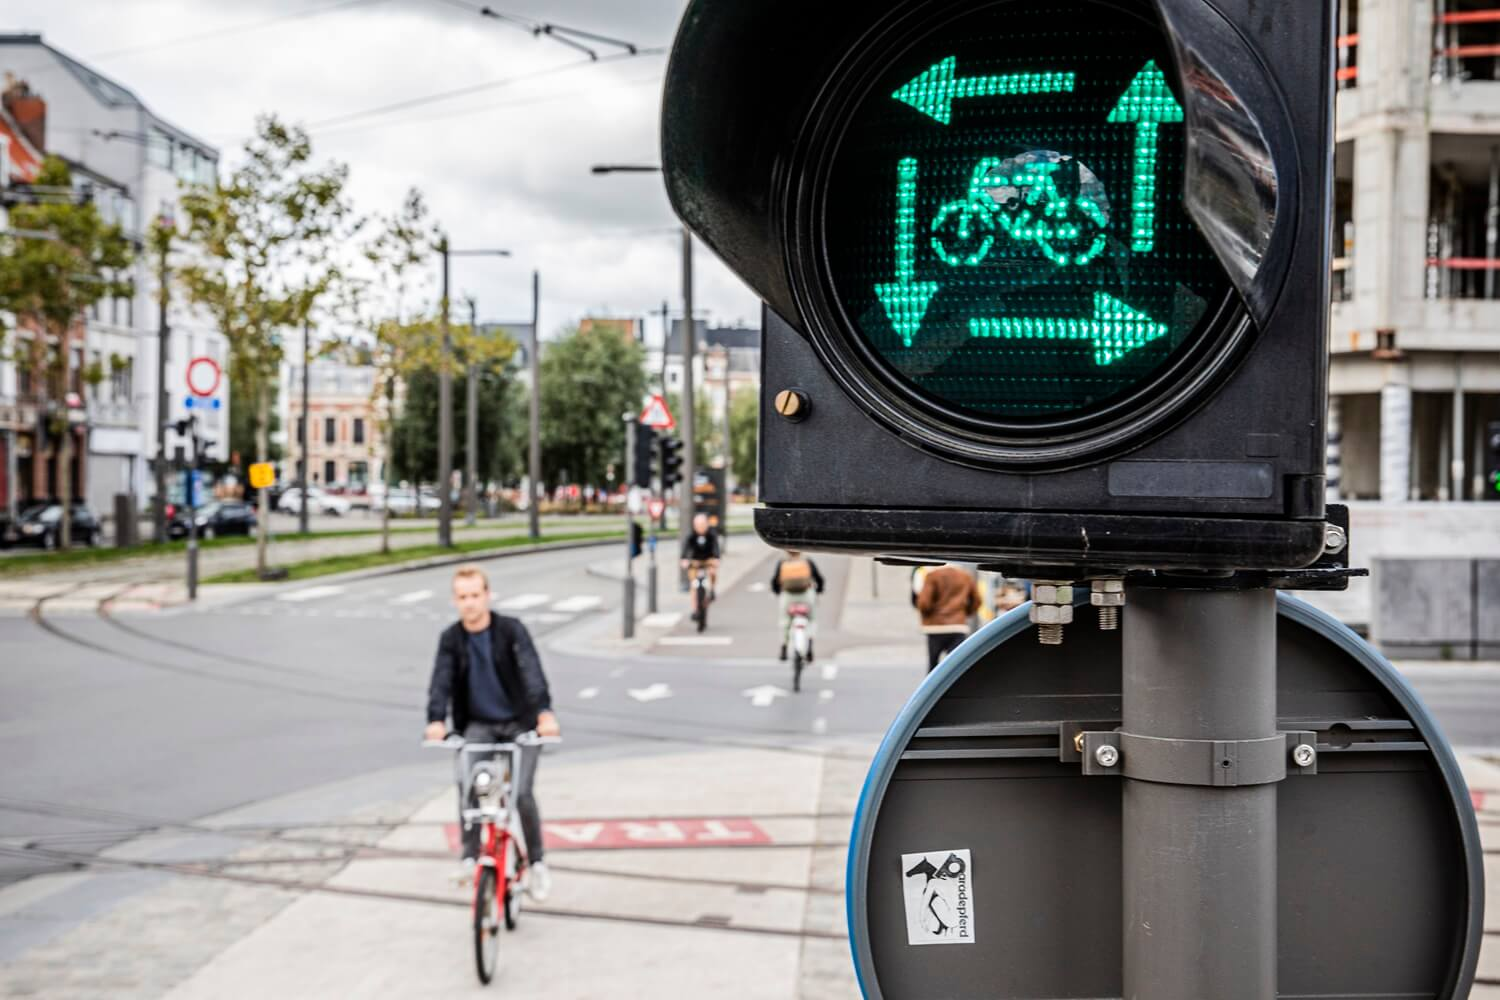
\includegraphics[height=4cm]{figures/verkeerssituaties48.jpg}
        \caption{Montage van verkeerslichten.}\label{fig:verkeerslichten}
        \textbf{Bron}: uitgesneden uit\ \cite{RN39}
    \end{figure}
\end{minipage}
\begin{minipage}[t]{0.49\textwidth}
    \begin{figure}[H]
        \centering
        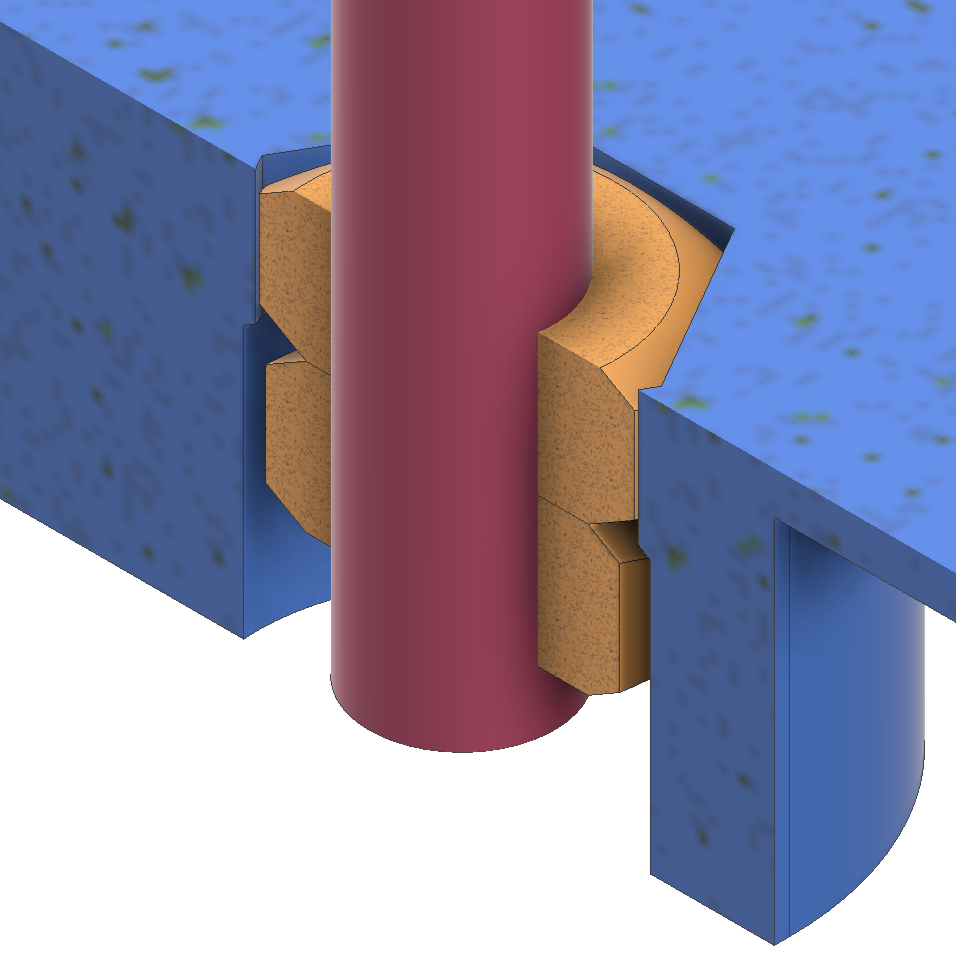
\includegraphics[height=4cm]{figures/InterlockingScrews.png}
        \caption{Tegengedraaide moeren}\label{fig:counterrotated}
    \end{figure}
\end{minipage}\\[12pt]
De bodemplaat is voorzien van verschillende gaten en uitsparingen zoals te zien in. Zo zijn er vier gaten voor de geleidestaven. Ook is er een groot centraal gat voor de loodschroef. Hierin past een lager van formaat ID:4mm, OD:8mm. Verder is er een uitsparing waar een eindeloopschakelaar past. Aan de rand is er een uitsparing waar de spuit in past. Rond deze uitsparing is er een verlaging waar de grepen van de spuit inpassen. Dit alles wordt met een klem vastgehouden doorheen de beweging. Deze klem past in de uitsparing en wordt vastegezet met twee M3 schroeven en de daarvoor voorziene gaten.
\\[12pt]\begin{minipage}[t]{0.49\textwidth}
    \vspace{0pt}
    \begin{figure}[H]
        \centering
        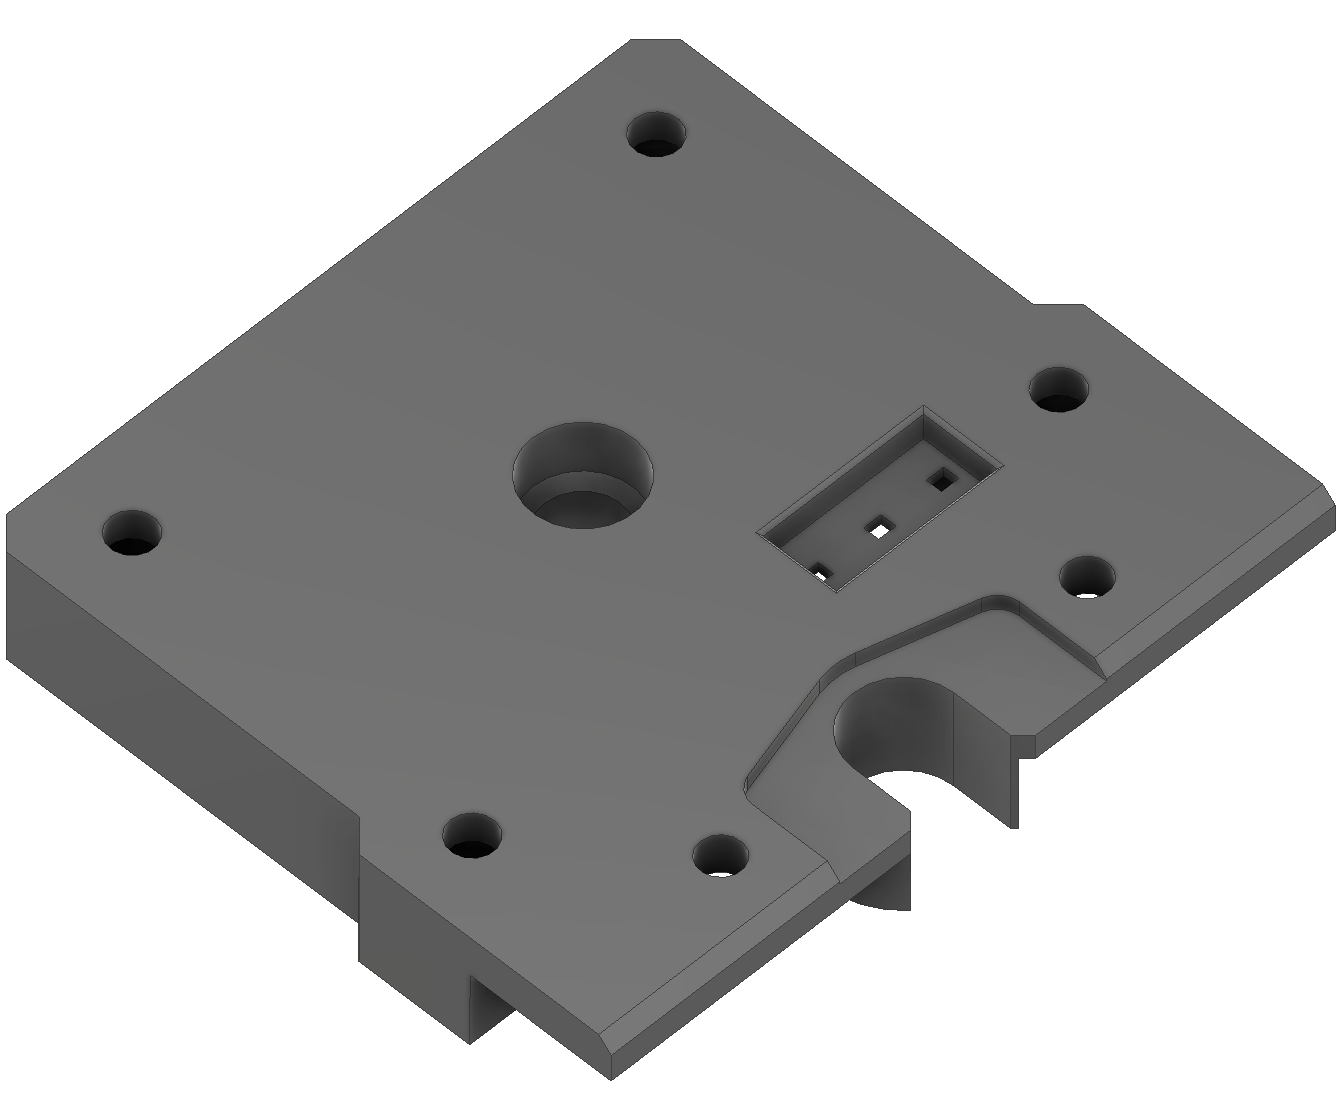
\includegraphics[height=4cm]{figures/Foundation_1_w.png}
        \caption{Bodemplaat.}\label{fig:bodemplaat}
    \end{figure}
\end{minipage}
\begin{minipage}[t]{0.49\textwidth}
    \vspace{0pt}
    \begin{figure}[H]
        \centering
        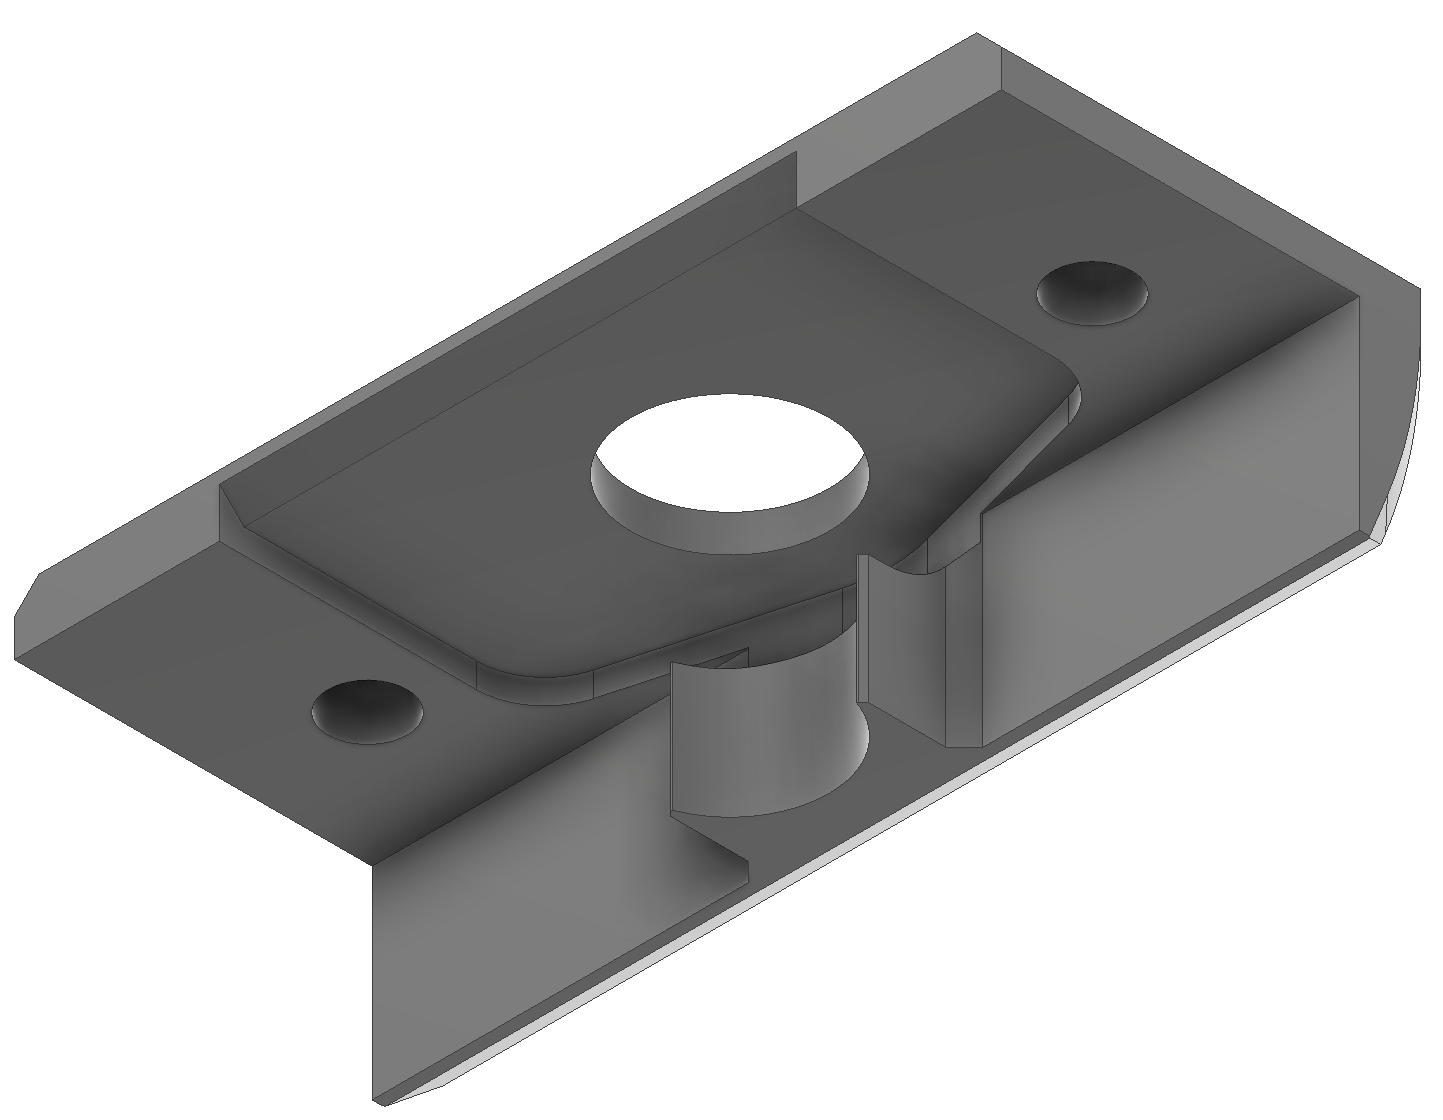
\includegraphics[height=4cm]{figures/Foundation_clamp_w.png}
        \caption{Klem zuiger}\label{fig:clamp}
    \end{figure}
\end{minipage}\\

\subsection{Tussenplaat en motorplaat}
Deze twee platen passen tussen de muurelementen. De tussenplaat vormt de grens tussen de askoppeling en de zuigerkamer. De motorplaat bevindt zich bovenaan en heeft een uitsparing voor een Nema 8 stappermotor die met M2 schroeven bevestigd wordt. 
\\[12pt]\begin{minipage}[t]{0.49\textwidth}
    \vspace{0pt}
    \begin{figure}[H]
        \centering
        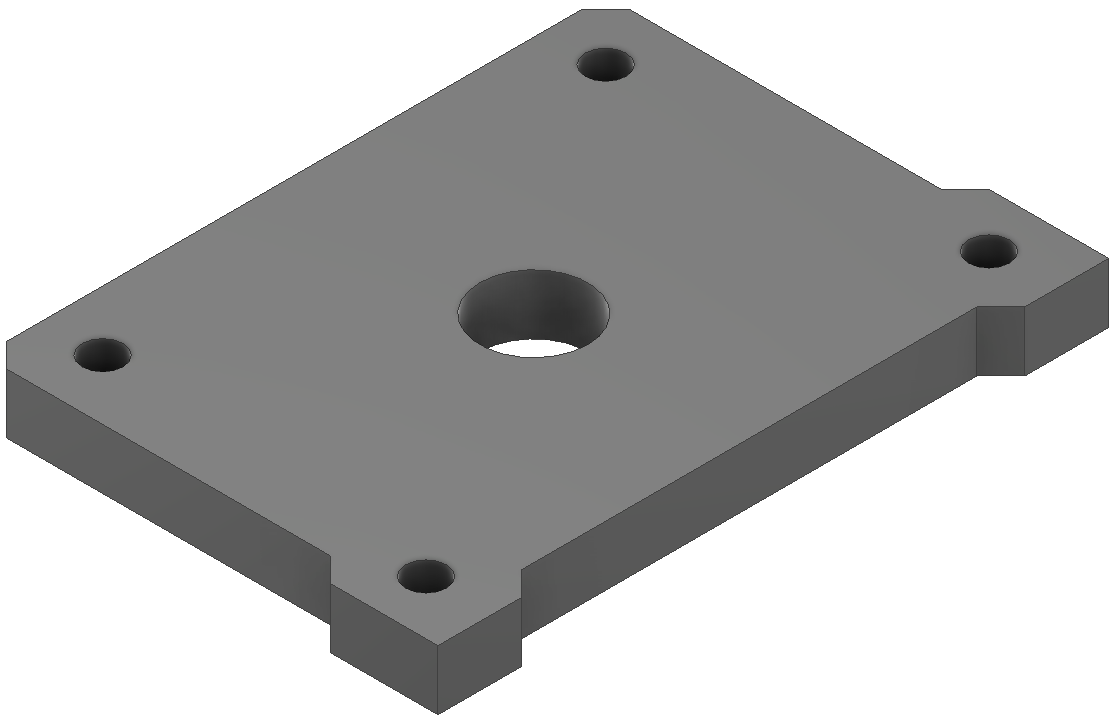
\includegraphics[width=0.65\textwidth]{figures/Topp_Wall_w.png}
        \caption{Tussenplaat.}\label{fig:tussenplaat}
    \end{figure}
\end{minipage}
\begin{minipage}[t]{0.49\textwidth}
    \vspace{0pt}
    \begin{figure}[H]
        \centering
        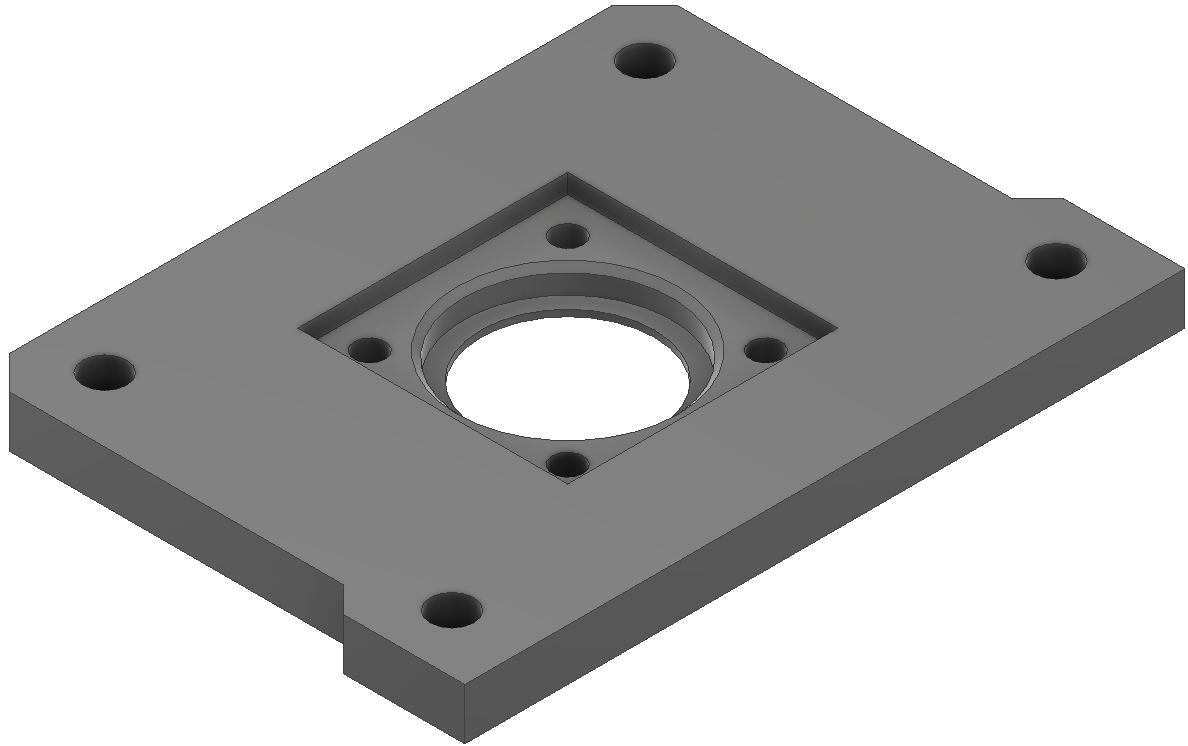
\includegraphics[width=0.65\textwidth]{figures/motor_mount_wide.png}
        \caption{Motorplaat.}\label{fig:motorplaat}
    \end{figure}
\end{minipage}\\

\subsection{Loodschroef, motor en askoppeling}\label{sec: motor}
Voor de loodschroef is een schroef van het type T4 gekozen met een spoed en lood van 1mm. Er is een moer gekozen zonder anti-terugslag mechanische. Terugslag zal namelijk programatisch geëlimineerd worden. De moer heeft 3 gaten, van het formaat M3, die gebruikt worden om de geleideslede te bevestigen.
\\[12pt]De motor is een Nema 8 stappermotor van het type 8HS15--0604D met een maximaal koppel van 0.4N-cm en een stapgrootte van 1.8° per stap. In eerste instantie werd in het ontwerp een zwakkere motor gebruikt (0.2N-cm). Deze mistte echter te veel stappen en is dus vervangen.
\\[12pt]De askoppeling is een flexibele askoppeling van het type 4mm-4mm. Er is gekozen voor een flexibele askoppeling omdat, door het stuikgedrag van PLA na het bevestigen van de moeren, de assen niet meer perfect uitgeliend zijn.

\subsection{Geleideslede}
De geleideslede is het onderdeel dat de zuiger aanstuurt. Deze bestaat uit 3 onderdelen. Het centrale onderdeel, de effectieve slede, is bevestigd met 3 M3 schroeven aan de moer van de loodschroef. Zoals te zien in\ \autoref{fig:CarriageDemonstration} heeft de geleideslede hoge wanden. Deze aanpassing is later in het ontwerp gemaakt toen uit de initiële testen bleek dat de slede de neiging had om to oscilleren. Dit is nu sterk verminderd. Het grotere oppervlak zorgt echter wel voor meer weerstand maar tegenover de zuiger is dit verwaarloosbaar.
\\[12pt]Aan de slede is ook een klem bevestigd. Deze is bevestigd met geleidestaven van 55mm met een bevestiging, gelijkaardig aan die van de grote geleidestaven. De klam bestaat uit twee delen. Het eerste deel heeft een gleuf waar de zuiger in wordt geschoven. De handvaten van de zuiger houden deze op zijn plaats bij de opwaartse slag. Daarna wordt er een bovenste klem bevestigd. Deze klemt de zuiger volledig in. De twee klemmende delen kunnen vervangen worden naargelang de dimensies van de zuiger.
\\[12pt]\begin{minipage}[t]{0.39\textwidth}
    \vspace{0pt}
    \begin{figure}[H]
        \centering
        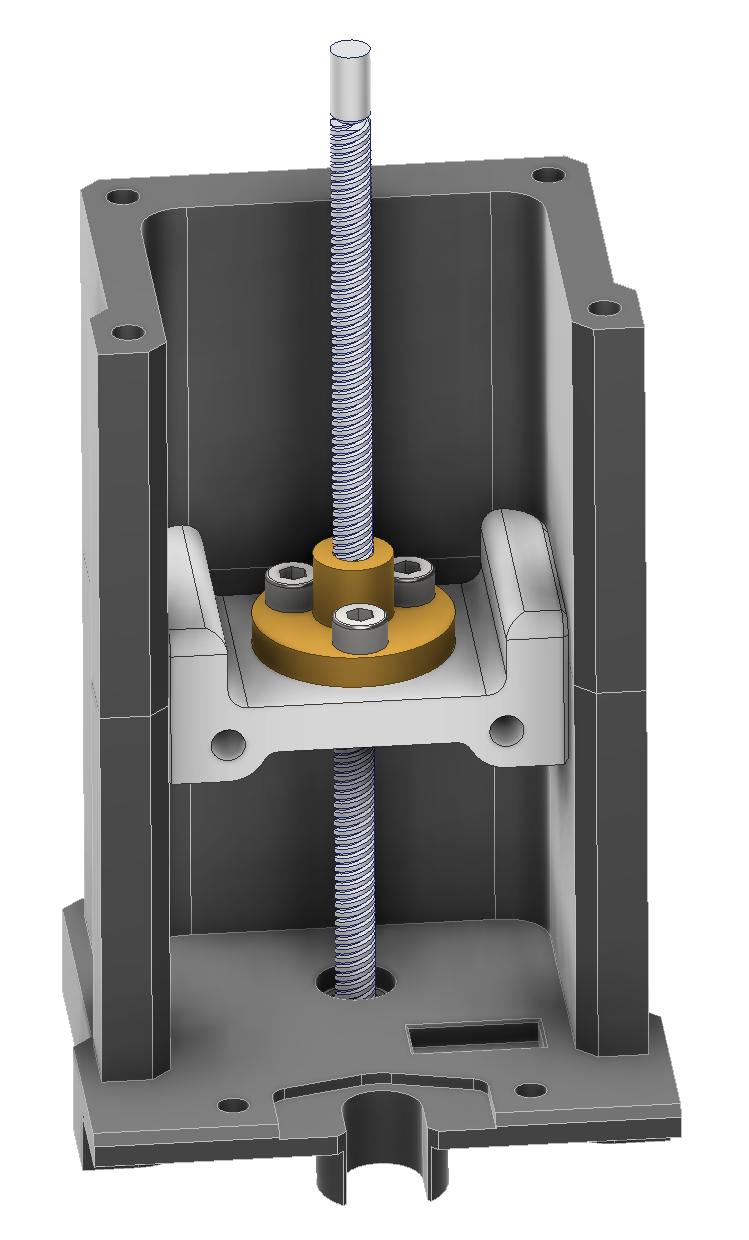
\includegraphics[width=0.65\textwidth]{figures/CarriageDemonstration.png}
        \caption{De geleideslede tussen de muren.}\label{fig:CarriageDemonstration}
    \end{figure}
\end{minipage}
\begin{minipage}[t]{0.59\textwidth}
    \vspace{0pt}
    \begin{figure}[H]
        \centering
        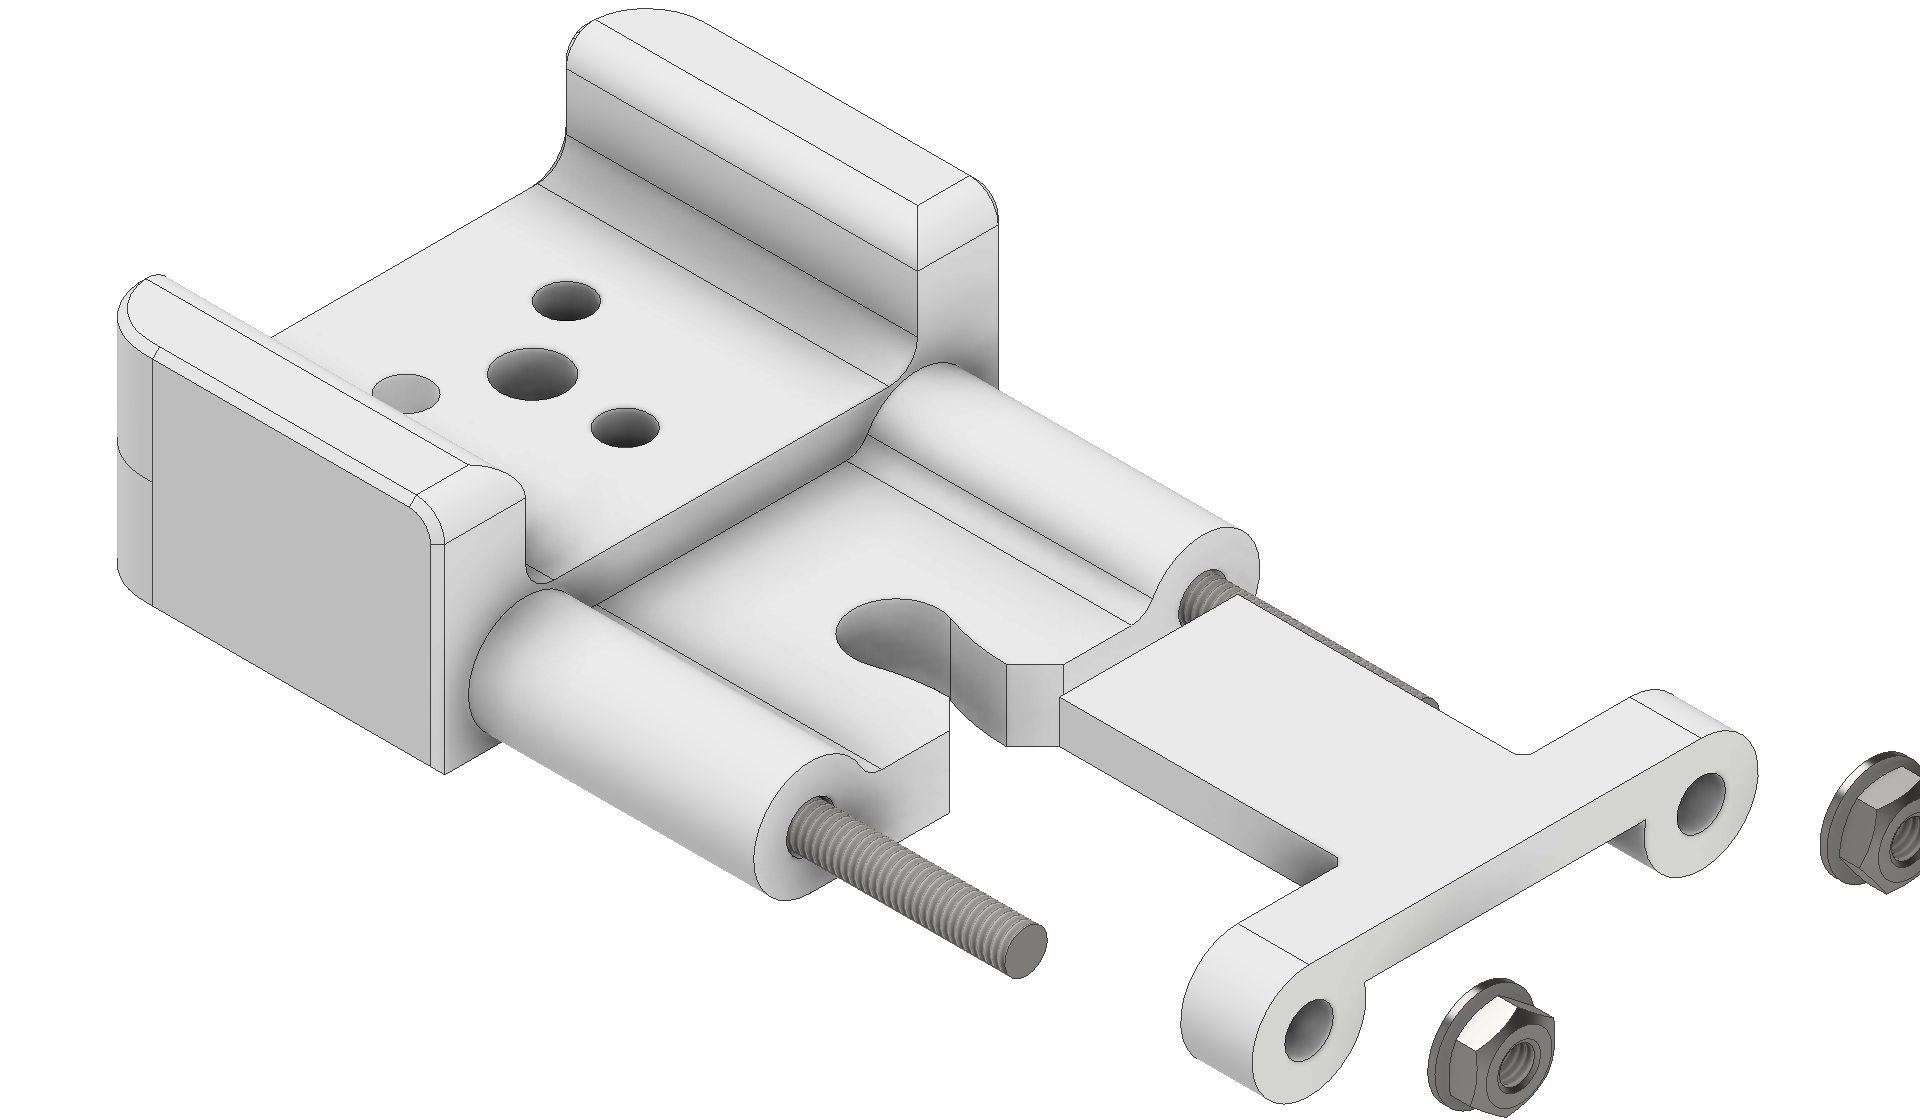
\includegraphics[width=0.85\textwidth]{figures/CarriageAndClamp.png}
        \caption{De geleideslede. Inclusief de samengestelde zuigerklem.}\label{fig:CarriageAndClamp}
    \end{figure}
\end{minipage}\\

\subsection{Zuiger}
Voor de zuiger is gekozen voor standaard verkrijgbare spuiten met een volume van 1000$\mu$l. Deze spuit kan vervangen worden naargelang de gebruikssituatie. In het huidige ontwerp wordt er gewerkt met een spuit van het merk DB, type ISO 7886--1 Luer Slip 1ml. Doordat deze spuiten courant beschikbaar zijn kunnen ze, indien nodig, vervangen worden.
Een belangrijk aspect bij de keuze voor een bestaande spuit was het feit dat ge-3D-print filament niet luchtdicht is en dus geen stabiel vacuum zou kunnen onderhouden. Door een bestaande spuit te gebruiken kan deze bron van fouten deels verholpen worden.

\section{Elektronica ontwerp}
\subsection{Componentenlijst}
\begin{table}[H]
    \begin{tabular}{l|c|c}
        \textbf{Component} & \textbf{Type} & \textbf{Aantal} \\
        \hline
        Motor & Nema 8 (8HS15--0604D)& 1 \\
        Motor driver & BigTreeTech TMC2209 & 1 \\
        Microcontroller & ESP32-WROOM-32 & 1 \\
        eindeloopschakelaar & Micro Limit switch & 1 \\
        5V Voeding & Vrij te kiezen\footnotemark & 1 \\
        \hline
    \end{tabular}
    \caption{Componentenlijst.}\label{tab:componentenlijst}
\end{table}
\footnotetext{{$I_{bron} > 1.7A$}}
\subsection{Motor}
Zoals eerder vermeld in \autoref{sec: motor} is er gekozen voor een Nema 8 motor met een koppel van 0.4N-cm. Dit koppel is voldoende om één zuiger aan te drijven. Een Nema 8 motor is een motor met een relatief klein formaat en past daardoor binnen de afmetingen van het ontwerp. Zoals reeds vernoemd was het ontwerp initieel uitgevoerd met een Nema 8 motor met een koppel van 0.2N-cm. Dit bleek echter te weinig. Deze motor kon de gewenste aspiratiesnelheden niet bereiken en kon de weerstand van de zuiger en geleideslede niet overwinnen.
\\[12pt]De motor heeft 4 aansluitingen (2 per fase) en wordt in dit ontwerp in een open lus gestuurd. Om de fouten te minimaliseren wordt er aangeraden om de pipet zo vaak mogelijk naar de nulpositie te brengen. Hier is een eindeloopschakelaar voor voorzien.
\subsection{Driver}
Er is gekozen voor een TMC2209 stappermotor driver. Deze driver heeft een belangrijk voordeel. Deze kan gebruik maken van zogeheten \"StealthChop\" technologie. Dit zorgt voor een stillere motorwerking. Belangrijk voor deze toepassing is er een soepeler motorverloop met hogere nauwkeurigheid en minder ruis. Een constante pipetteersnelheid is een belangrijke factor in de nauwkeurigheid van de handling. Anderzijds zorgt de het verbeterde stroomprofiel ook voor een verhoging van het effectieve koppel van de motor.\ \cite{RN45}
\subsection{Microcontroller}
Voor de controller is er een ESP32-WROOM-32 gekozen. Deze is voornamelijk gekozen vanwege de hoge kloksnelheid van 80 MHz tot 240 MHz (zie\ \cite{RN46}). Door deze hoge kloksnelheid kan de controller zeer snel stap-signalen naar de driver sturen. Dit is interessant omdat de TMC2209 driver bij kleinere micorstepping een steeds vlotter stroomverloop kan voorzien. Bij micorstepping is de maximale snelheid van de motor echter lager bij een constant aantal stappen/s. Deze stapsnelheid is beperkt door de klok van de controller. De ESP32-WROOM-32 kan de motor dus aan een hoger toerental aandrijven dan meeste andere controllers. Verder is de controller relatief goedkoop (circa €10) en makkelijk te verkrijgen.
\subsection{Aansluiting}
\begin{figure}[H]
    \centering
    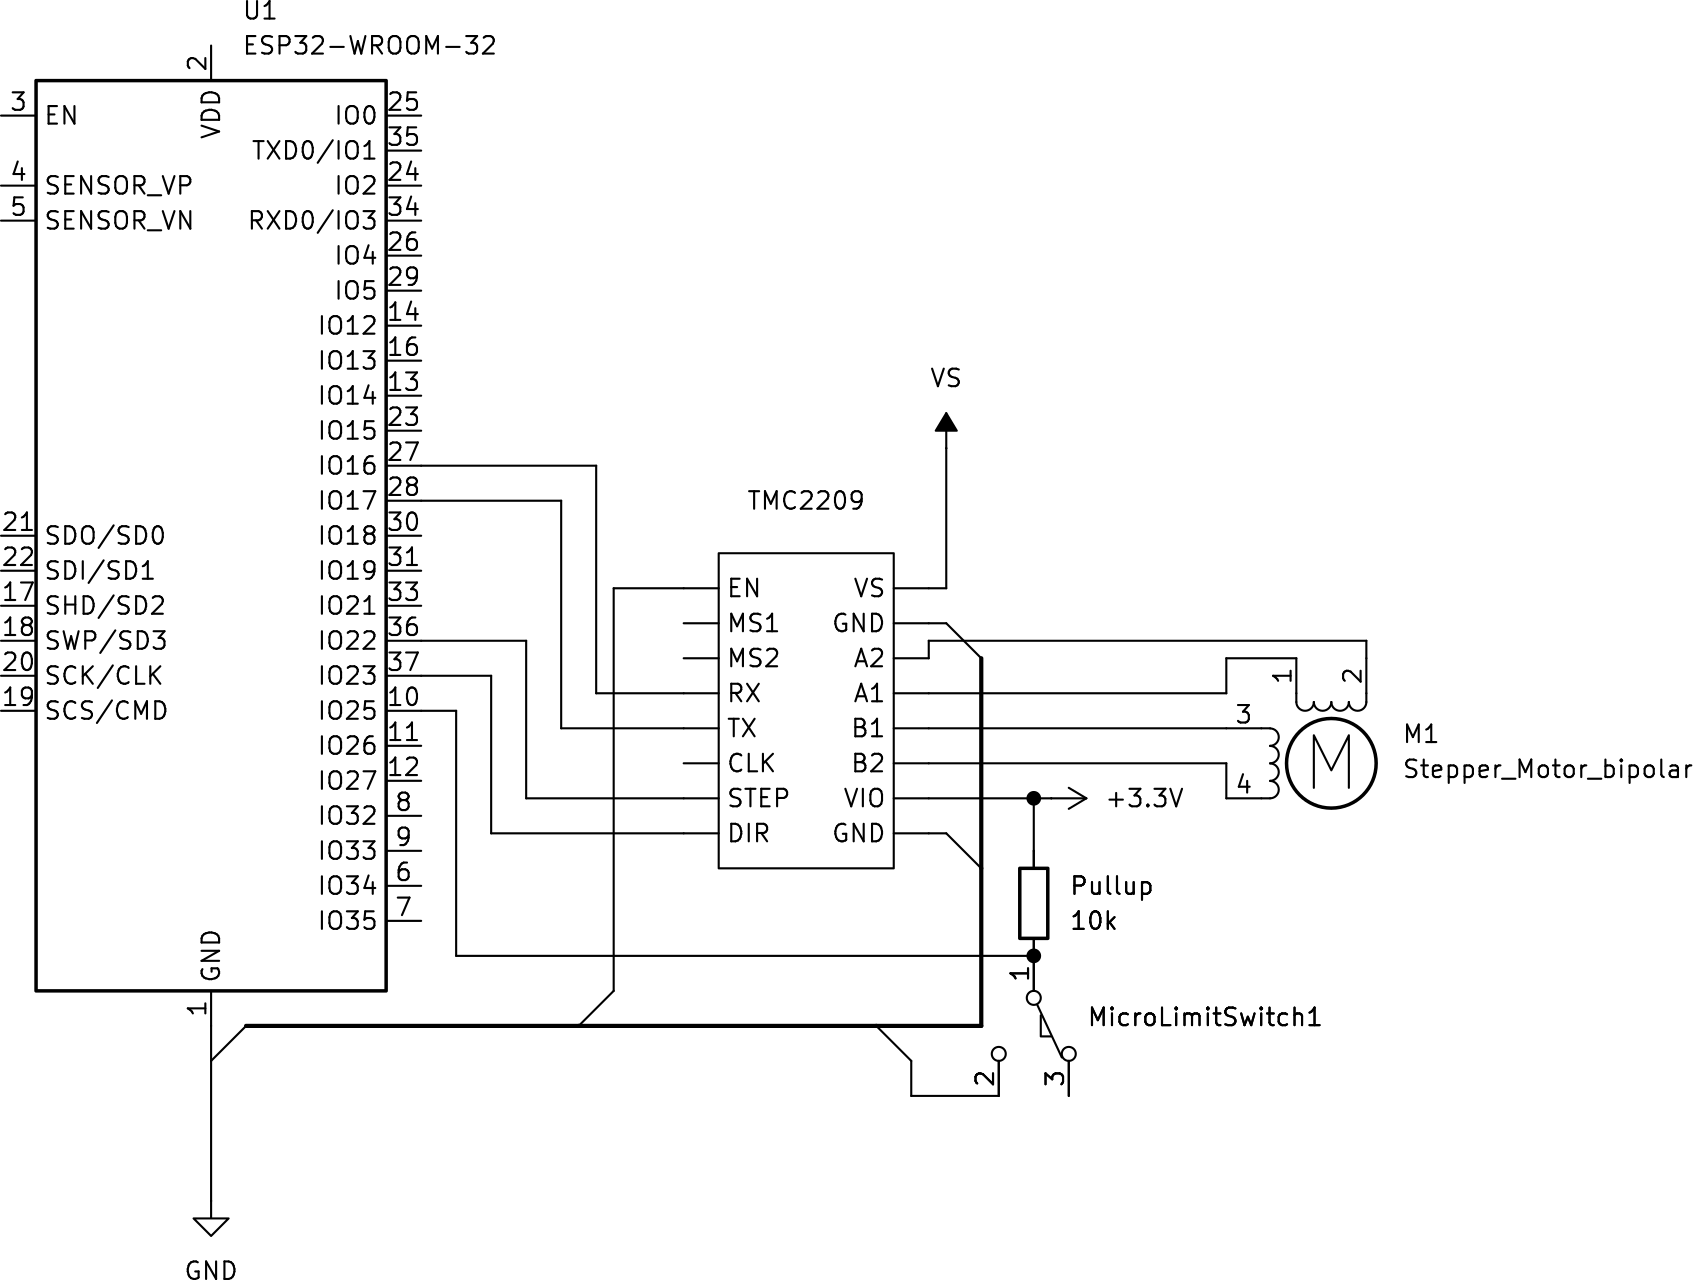
\includegraphics[width=0.85\textwidth]{figures/Wiring_BW.png}
    \caption{Schema van de aansluiting.}\label{fig:schematische_aansluiting}
\end{figure}
De aansluiting van de elektronische componenten gebeurt zoals in \autoref{fig:schematische_aansluiting} te zien is. De motor wordt aangesloten op de TMC2209 driver. Deze driver wordt aangesloten op de ESP32-WROOM-32. De eindeloopschakelaar wordt ook aangesloten op de ESP32-WROOM-32. De voeding van de motor en driver is een 5V voeding. Deze voeding kan vrij gekozen worden, zolang deze maar voldoende stroom kan leveren. De voeding van de ESP32-WROOM-32 kan ook vrij gekozen worden, zolang deze tussen de 3.3V en 5V ligt. De aansluiting van TX en RX aan de driver is vrijblijvend, maar is wel aangeraden aangezien hiermee de stroomlimiet en microstapgrootte geconfigureerd kunnen worden.

\section{Software ontwerp}
\begin{figure}[H]
    \centering
    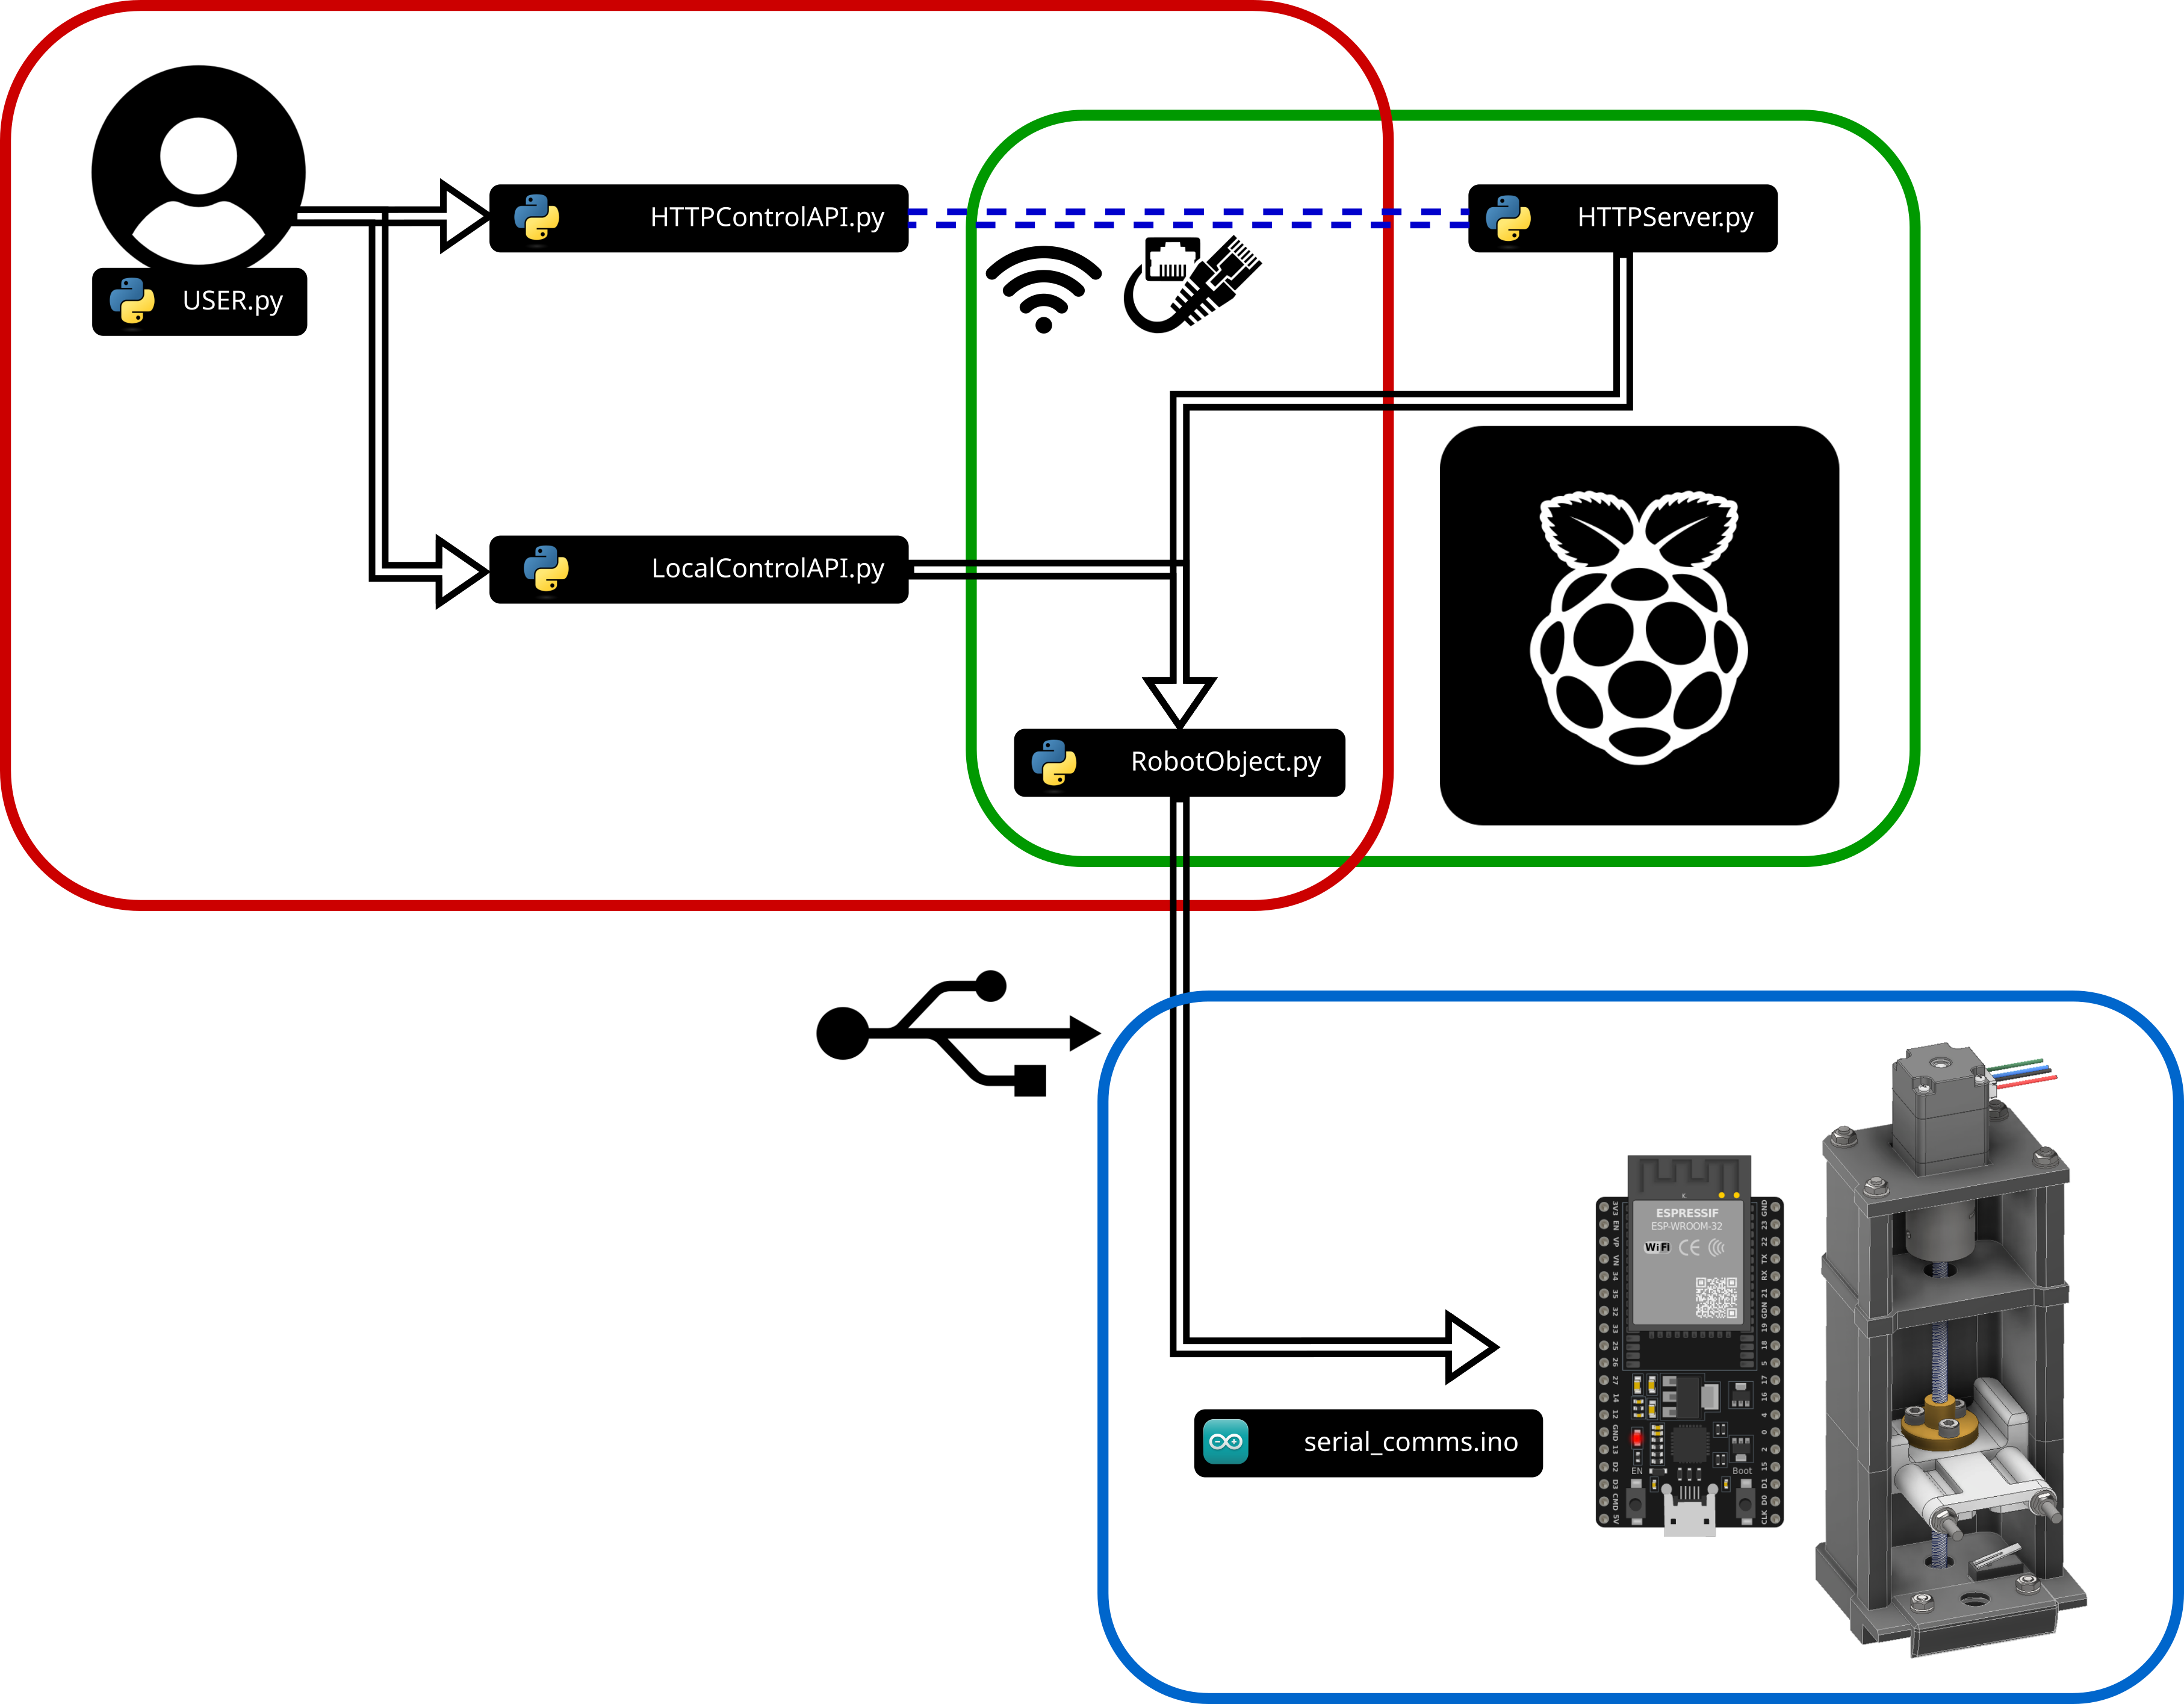
\includegraphics[width=0.85\textwidth]{figures/Flowchart.png}
    \caption{Flowchart communicatie.}\label{fig:Flowchart}
\end{figure}
